\subsection{\texorpdfstring{\(\mathbf{C}\) 的拓扑}{复数域 C 的拓扑}}

映射 \((x, y) \to x + iy\) （实平面 \(R^{2}\) 到 C 上的）是双射；借助这个双射，我们可以把 \(R^{2}\) 的拓扑转移到 C 上（参看第六章，§ 1，第 5 号）。这样在 C 上定义的拓扑与 C 的域结构相容（第三章，§ 6，第 7 号），因为它与 C 的环结构相容（第六章，§ 1，第 5 号），并且由 (3)，1/z 在 C 中 o 的余集 \(C^{*}\) 上连续。

若把集合 C 赋以上述拓扑以及前面（第 1 号，定义 1）定义的域结构，我们就在 C 上定义了拓扑域的结构（第三章，§ 6，第 7 号）；以后每当我们谈到 C 的拓扑时，所指的总是上述拓扑。

今后我们一般把作为拓扑空间的集合 C 与 \(R^{2}\) 等同起来；此时 C 的子域 R 与 \(R^{2}\) 的横轴等同，因此后者称为实轴；同样地，纵轴称为虚轴（注意它不是 C 的子域）。以 o 为端点、方向比为 (1, o) 的射线（与 \(R_{+}\) 等同）称为正实半轴；与之相反、同以 o 为端点、方向比为 (-1, o) 的射线称为负实半轴。

为作图说明起见，我们利用 \(R^{2}\) （初等解析几何中众所周知）借平面的点所作的表示，平面内画有两条互相垂直的坐标轴，分别表示 C 的实轴与虚轴（图 7）。

如同在每个拓扑域中一样，每个带复系数的 n 个复变量的有理函数，在 \(C^{n}\) 中每个使分母不为零的点处连续。

\pandocbounded{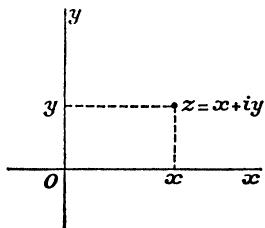
\includegraphics[keepaspectratio]{images/part001_cf49e1ad.jpg}}\\
图 7。

置换 \(z' \to \overline{z}\) （\(\mathbf{C}\) 的）是连续的，因此它是拓扑域 \(\mathbf{C}\) 的一个自同构。

事实上，它是拓扑域 C 中除恒等自同构外唯一的自同构（见习题 4）。

函数 \(\mathcal{R}(z)\) 、\(\mathfrak{J}(z)\) 正是 \(\mathbf{R}^2\) 到它的各因子上的投影，因此是连续的；绝对值 \(|z|\) 亦然，因为它是点 \((x,y)\) （在 \(\mathbf{R}^2\) 中）的欧氏范数（第六章，§ 2，第 1 号）。

绝对值的性质给出了 \(\mathbf{C}\) 的拓扑与其域结构相容这一事实的另一个证明（参看第九章，§ 3，第 2 号）；\(z + z'\) 的连续性由三角不等式 \(|z + z'| \leqslant |z| + |z'|\) 得出；\(zz'\) 的连续性由关系式

\[
\begin{array}{r l} | z z ^ {\prime} - z _ {0} z _ {0} ^ {\prime} | & = | z _ {0} (z ^ {\prime} - z _ {0} ^ {\prime}) + (z - z _ {0}) z _ {0} ^ {\prime} + (z - z _ {0}) (z ^ {\prime} - z _ {0} ^ {\prime}) | \\ & \leqslant | z _ {0} | \cdot | z ^ {\prime} - z _ {0} ^ {\prime} | + | z _ {0} ^ {\prime} | \cdot | z - z _ {0} | + | z - z _ {0} | \cdot | z ^ {\prime} - z _ {0} ^ {\prime} |; \end{array}
\]

得出；最后，\(z^{-1}\) 的连续性由关系式

\[
\left| z _ {0} ^ {- 1} - z ^ {- 1} \right| = | z | ^ {- 1}. \left| z - z _ {0} \right|. \left| z _ {0} \right| ^ {- 1}.
\]

